%
% Capítulo 2
%
\chapter{Problem Description And Proposed Solution} \label{cap:problem_description}

Current blood donation workflow faces a set of challenges like screening time for more complex cases, since higher complexity cases may require cross-checking information about drug and pathology interaction, a process that, beyond being time-consuming,  may lead to imprecisions with severe consequences. Currently upon form changes the previously printed forms are disregarded, this process can be expedited by supporting a digital form that can be easily updated, helping IPO reduce its paper consumption.

These challenges can be met by employing a dynamic form, in digital format, that shows relevant follow up questions according to the potential donor's answers, thus collecting relevant information, that would otherwise need to be obtained during the medical screening.
This solution raises a set of questions such as:
\begin{itemize}
	\item What data structure is appropriate to describe the form's structure and flow/logic - 
	the questions order, possible answer values, what answers trigger or suppress follow-up questions;
	\item How will the form's rule be enforced in a way that doesn't force code implementation changes upon form structure changes - the frontend should be able to show and compute various forms and its unfeasible to change the frontend implementation upon every form structure change.
\end{itemize}

Upon form submission, the information supplied by the potential donor, or automatically obtained, can be automatically cross-checked against IPST guidelines for drug and pathology interaction with blood donation.
This solution raises a set of questions such as:
\begin{itemize}
	\item How are the potential donor's drug and disease information validated - the number of available drugs and possible diseases might be too large for real time validation, when the user is inputting that information into the form;
	\item Are the IPST guidelines available in a machine readable format that make it feasible to be cross-checked against the form's answers - to our knowledge, the guidelines are available in pdf and printed format, sometimes drugs/pathologies are individually mentioned and sometimes grouped in a family (ie there's no mention of aspirin in the 2022 manual, being replaced by Non Steroidal Anti Inflammatory, the family of drugs this medication belongs to).
\end{itemize}

The digital form structure and flow, pathology/drug interaction, and terms of service information should be updatable in the back-office. 

This solution raises a set of questions such as:
\begin{itemize}
	\item How can the form structure and flow be visualized intuitively - the user changing the form shouldn’t need to know anything about its implementation but still be able to identify and change its structure and flow;
	\item How will the drug/pathology interaction be updated - will a user manually insert information in the platform or can this information be requested via a web-service. 
\end{itemize}

Beyond these specific challenges the platform will have to employ multiple types of users, each with a given set of accesses, there are multiple ways of implementing role-based access control, each with pros and cons.

\section{Proposed Solution}

In order to solve the challenges listed above, we have developed DADIVA IPO.

DADIVA IPO is a web platform that allows blood donation services to decrease the screening time of blood donation candidates via a digital, updateable and dynamic form as well as automatic interaction verification.

It is intended as an alternative to the current, and less versatile, paper form used by blood donation services in Portugal, such as Lisbon's IPO.

\subsection{Functional Requirements}
\begin{itemize}
	\item Donors should be able to quickly fill out a digital pre-donation form. The form should be adequate according to the current law, adaptable, and depend on the donor’s answers.
	
	\item Doctors should be able to find all relevant data on pathology and/or medication interactions with the donation in a digital format.
	
	\item Doctors and administrators should be able to access a back office used for customizing the pre-donation form and for updating the pathology and/or medication interaction information. The back office should also allow for user management.
	
	\item Google-like search and results by relevance - Search should be as simple as possible. There may be a need to increase the number of filters, but this complexity should be hidden. The results returned should be sorted based on relevance.
\end{itemize}

\subsection{Non-Functional Requirements}
\begin{itemize}
	\item Intuitive user experience through a simple and practical user interface.
	
	\item Responsive design that ensures a good user experience both on desktop and mobile.
	
	\item Complete and thorough documentation.
	
	\item Unit and integration testing with sufficient coverage to ensure confidence that the system is working without flaws.
	
	\item Good software engineering practices to ensure the fast development of the system.
\end{itemize}

\subsection{Use Cases}\label{sec:use_cases}
With the requirements listed above, we have identified the use cases that the platform
shall support. A use case is a written description of how users will perform tasks on
a system. It outlines, from the user's perspective, the behavior of the system as it
responds to a request. This approach attempts to predict the users of the platform, their allowed actions and objectives, and how the platform should respond to each action.
The use cases are divided into three categories, each representing one type of user.
The Donor use case is presented in Figure ~\ref{fig:donor_use_case}.

\begin{figure}[h]
	\begin{center}
		\resizebox{100mm}{!}{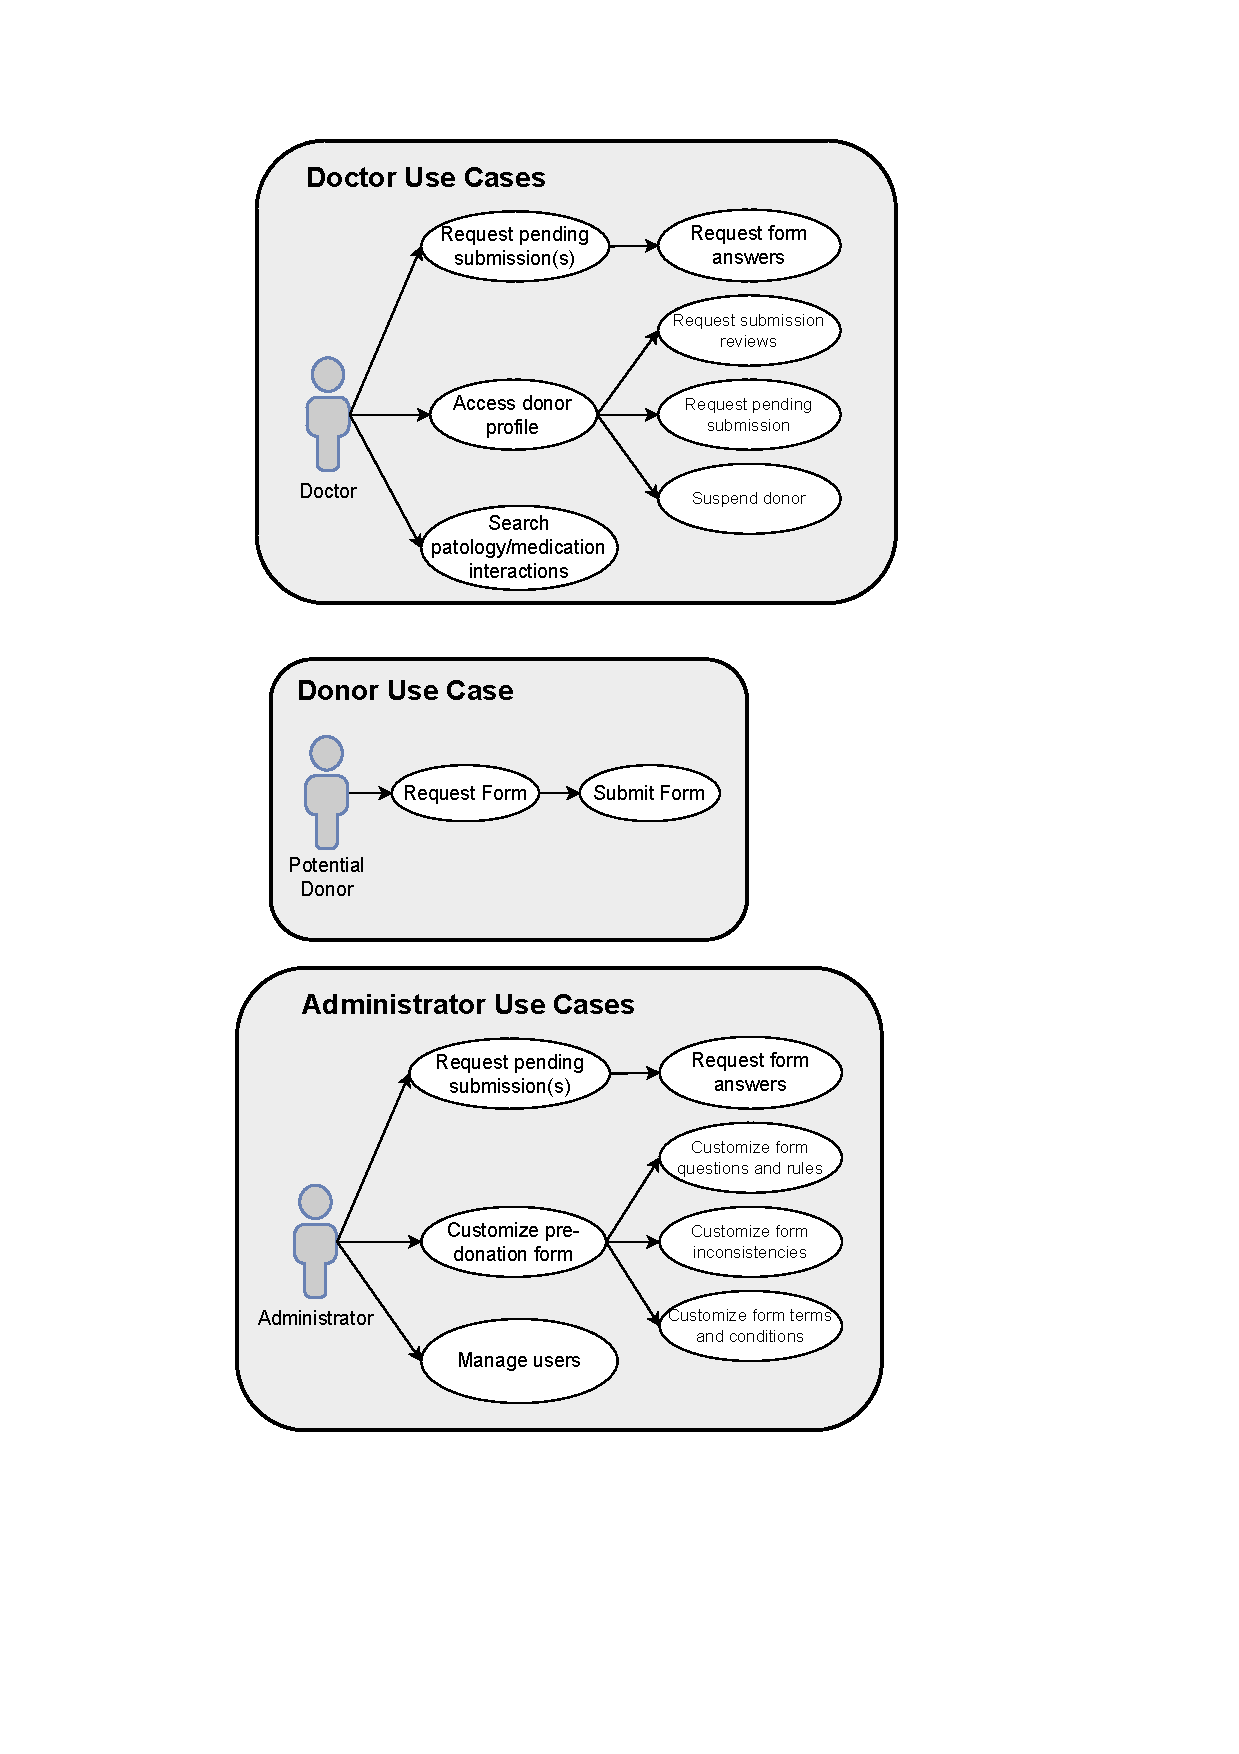
\includegraphics[trim={0 540 70 0},clip]{./figures/useCases.pdf}}
	\end{center}
	\caption{Donor use case.}\label{fig:donor_use_case}
\end{figure}
The donor user can request the current form and can submit their form responses.

\pagebreak

After a donor submits their form responses a doctor user will be able to access their answers by searching by the user's unique id as presented in Figure~\ref{fig:doctor_use_case}.

\begin{figure}[h]
	\begin{center}
		\resizebox{100mm}{!}{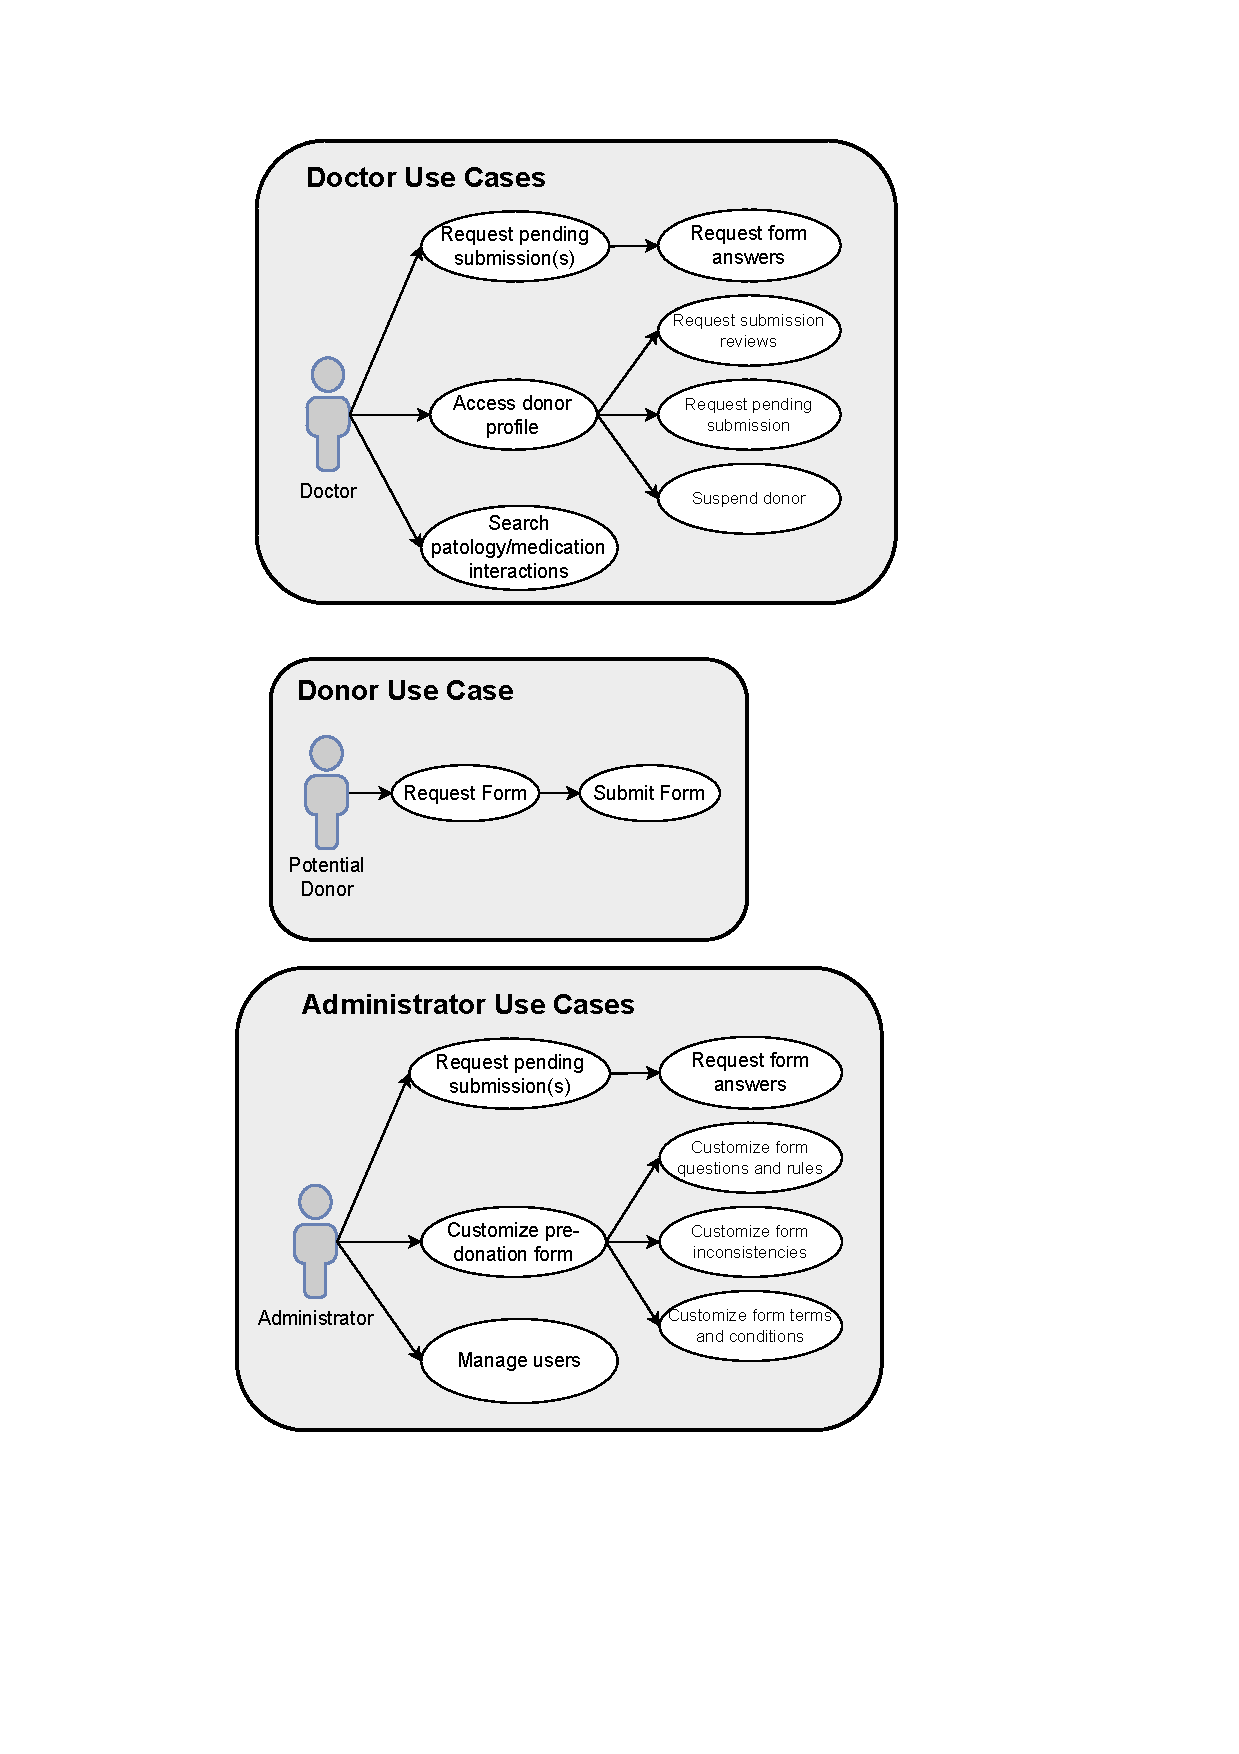
\includegraphics[trim={0 330 70 220},clip]{./figures/useCases.pdf}}
	\end{center}
	\caption{Doctor use case.}\label{fig:doctor_use_case}
\end{figure}

Furthermore the doctor user is able to search for pathology/medication interactions to resolve any inquiries that might appear during the screening.

Finally the administrator user can update the form structure and flow, update the interaction information and manage the platform's users.
The administrator use case is presented in Figure ~\ref{fig:administrator_use_case}.
\begin{figure}[h]
	\begin{center}
		\resizebox{100mm}{!}{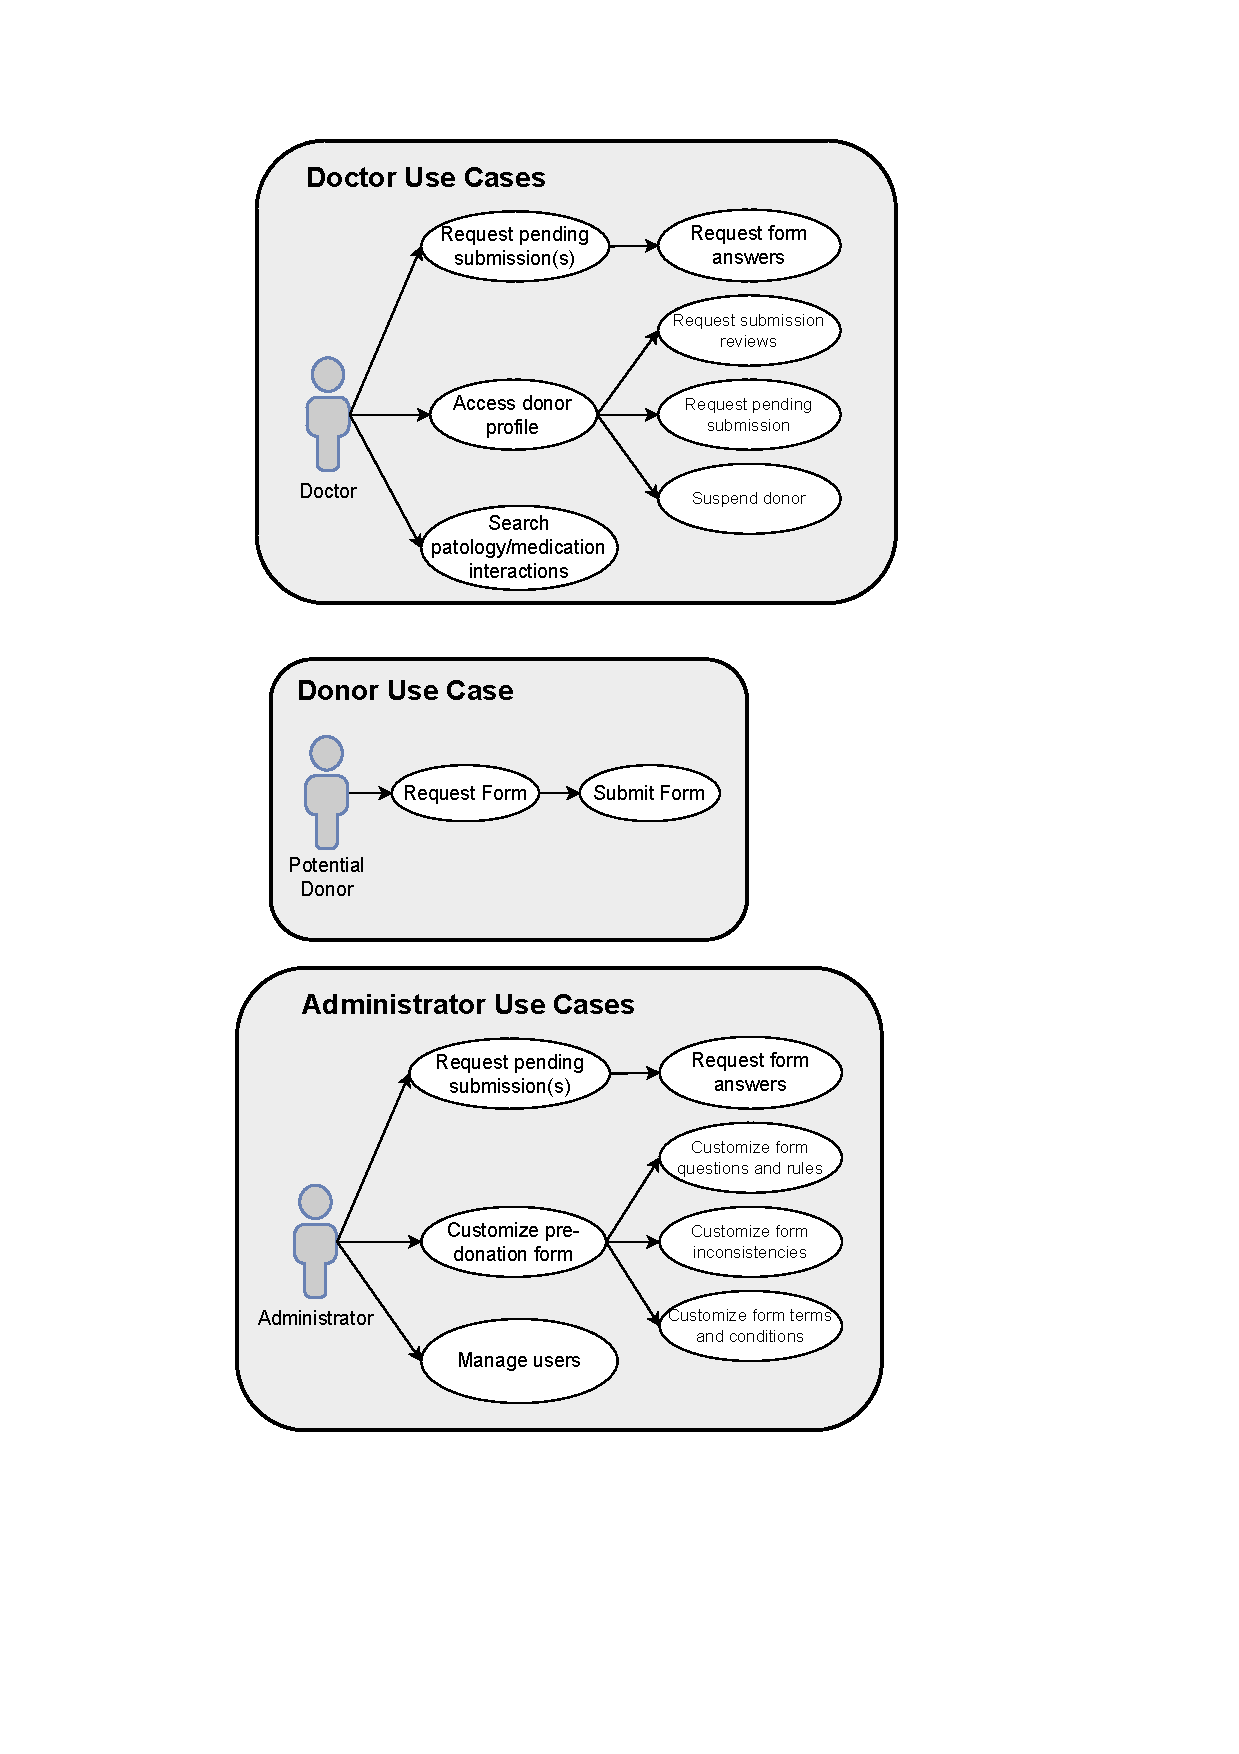
\includegraphics[trim={0 0 0 450},clip]{./figures/useCases.pdf}}
	\end{center}
	\caption{Administrator use case.}\label{fig:administrator_use_case}
\end{figure}